\documentclass[11pt,a4paper]{article}

%
%  Title:  "Filesystem-as-Pipe":
%          Extending Unix File Abstraction from Interface to
%          Composition for AI Agent Orchestration
%

\usepackage{fontspec}
\usepackage{geometry}
\usepackage{amssymb}
\usepackage{textcomp}
\usepackage{booktabs}
\usepackage{longtable}
\usepackage{multicol}
\usepackage{enumitem}
\usepackage{xcolor}
\usepackage{listings}
\usepackage{tcolorbox}
\usepackage{hyperref}
\usepackage{fancyhdr}
\usepackage{titling}
\usepackage{abstract}
\usepackage{caption}
\usepackage{subcaption}
\usepackage{pgfplots}
\pgfplotsset{compat=1.18}
\usepackage{tikz}
\usetikzlibrary{
  arrows.meta,
  positioning,
  shapes.geometric,
  shapes.multipart,
  calc,
  chains,
  fit,
  matrix,
  backgrounds,
  decorations.pathreplacing
}

\geometry{margin=1in, top=1.2in, bottom=1.2in}
\setmainfont{DejaVu Serif}
\setsansfont{DejaVu Sans}
\setmonofont{Hack}[Scale=0.88]

\definecolor{citegreen}{HTML}{2D7D46}
\definecolor{codebg}{HTML}{F5F5F5}
\definecolor{ruleline}{HTML}{CC3333}
\definecolor{actionline}{HTML}{3377CC}

\lstdefinestyle{python}{
  language=Python,
  basicstyle=\small\ttfamily,
  backgroundcolor=\color{codebg},
  frame=single,
  numbers=left,
  numberstyle=\tiny,
  breaklines=true,
  columns=fullflexible,
}

\lstdefinestyle{yaml}{
  basicstyle=\small\ttfamily,
  backgroundcolor=\color{codebg},
  frame=single,
  breaklines=true,
  columns=fullflexible,
}

\lstdefinestyle{bash}{
  basicstyle=\small\ttfamily,
  backgroundcolor=\color{codebg},
  frame=single,
  breaklines=true,
}

\tcbuselibrary{skins, breakable, theorems}

\newtcolorbox{bluebox}[1][]{
  colback=blue!5!white,
  colframe=blue!70!black,
  arc=4pt,
  boxrule=1pt,
  left=6pt,
  right=6pt,
  top=4pt,
  bottom=4pt,
  #1
}

\newtcolorbox{redbox}[1][]{
  colback=red!5!white,
  colframe=red!70!black,
  arc=4pt,
  boxrule=1pt,
  left=6pt,
  right=6pt,
  top=4pt,
  bottom=4pt,
  #1
}

\hypersetup{
  colorlinks=true,
  linkcolor=blue!50!black,
  citecolor=citegreen,
  urlcolor=blue!50!black,
}

\pagestyle{fancy}
\fancyhf{}
\fancyhead[L]{\small Filesystem-as-Pipe}
\fancyhead[R]{\small \thepage}
\renewcommand{\headrulewidth}{0.4pt}

\title{
  \vspace{-1.5cm}
  \textbf{Filesystem-as-Pipe: \\
  Extending Unix File Abstraction from Interface to Composition \\
  for AI Agent Orchestration}
}
\author{Michael Conrad}
\date{May 2026}

\begin{document}

\maketitle
\thispagestyle{fancy}

\begin{abstract}
AI agents accumulate context rot---intermediate state from prior dispatch stages that persists past its useful lifetime in the orchestrator's context window, degrading behavioral compliance and decision quality. Advisory guidelines prohibiting this accumulation fail because agents rationalize around prohibitions: empirical studies show omission constraints decay from 73\% to 33\% compliance over 16 turns while commission constraints persist at 100\%. We propose the filesystem-as-pipe model: a ritual discipline where every \texttt{skill()} and \texttt{task()} call declares mandatory input and output artifact paths. The orchestrator holds only routing metadata---paths, scope, and next dispatch target---while sub-agents consume artifact content independently from the filesystem. This extends Piskala's ``files-are-all-you-need'' framework from the agent--world interface (files as the medium of interaction) to the orchestration layer (files as the medium of composition). The model requires no agent runtime modifications; it lives entirely in skill card design and guideline patterns. We support our claims with evidence from a 4.1~GB session trace of 6,764 real agent sessions---172K tool calls, 77K reasoning steps---revealing measurable patterns consistent with context rot: 83\% tool call size degradation, 1,416 unfinished reasoning steps, and near-zero cache hit ratios in long sessions. We present the pipe model, survey the enforcement strategy landscape showing the gap it fills, and propose empirical methodology for validating its effectiveness.
\end{abstract}

\section{Introduction}
\label{sec:introduction}

\subsection{Motivation}
Large language model (LLM) agents---systems that autonomously plan, call tools, and adapt across multi-turn interactions---operate within a fundamental structural constraint: the context window. This bounded workspace holds the agent's instructions, conversation history, tool definitions, and intermediate reasoning state. As sessions lengthen and task complexity grows, the content of this workspace degrades not only through token overflow but through a subtler mechanism: the agent's own prior stages---spec bodies it loaded to pass to sub-agents, guideline text it read for routing decisions, verification results from earlier pipeline stages---persist in context long after they are needed.

We term this \textbf{context rot}: the passive degradation of signal-to-noise ratio as intermediate state persists past its useful lifetime within the orchestrator's context window. Rot is the mechanism; the observable outcomes---compliance decay, behavioral regression, rationalization---are downstream effects. Both can exist with plentiful token budget---they are a signal-to-noise problem, not a space problem.

Existing approaches to preventing context accumulation rely on advisory guidelines: ``the orchestrator MUST NOT hold implementation context.'' These fail. Gamage~\cite{gamage2026} demonstrates that omission (prohibitive) constraints decay from 73\% compliance at turn 5 to 33\% at turn 16 in a 4,416-trial causal study. Potham~\cite{potham2025} shows a ``cost of compliance'' where safety principles degrade task success rate from 80\% to 14\%, and that apparent compliance often masks task incompetence rather than principled choice.

\subsection{Thesis}
We propose the \textbf{filesystem-as-pipe} model: a ritual discipline where every \texttt{skill()} and \texttt{task()} call in an agent's orchestration chain declares mandatory input and output artifact paths. The orchestrator holds only routing metadata---paths, authorization scope, and next dispatch target. Sub-agents consume artifact content independently from the filesystem. The orchestrator never reads artifact content.

This converts an omission constraint---``don't accumulate intermediate state''---into a commission constraint---``write artifact to path X before each dispatch.'' Gamage's framework predicts the latter persists at 100\% while the former decays to 33\%.

The pipe model extends Piskala's~\cite{piskala2026} ``files-are-all-you-need'' framework from the agent--world interface (files as the medium of interaction) to the orchestration layer (files as the medium of composition between dispatch stages). No agent runtime modifications are required; the discipline lives entirely in skill card design, artifact path conventions, and guideline patterns.

\subsection{Contributions}
This paper makes the following contributions:
\begin{enumerate}[nosep]
  \item \textbf{Context rot as a distinct failure mechanism}---intermediate state from the agent's own dispatches that persists past its useful lifetime, distinguished from external-context degradation studied in prior work.
  \item \textbf{Filesystem-as-pipe model}---mandatory artifact path declaration per dispatch as ritual enforcement against context rot.
  \item \textbf{Enforcement strategy classification}---four categories of agent instruction compliance mechanisms, demonstrating the gap the pipe model fills.
  \item \textbf{Empirical session trace analysis}---evidence from 6,764 real agent sessions revealing patterns consistent with context rot.
  \item \textbf{Extension of Piskala's framework}---from agent--world interface to orchestrator--sub-agent dispatch composition.
\end{enumerate}

\section{Context Rot: Mechanism and Evidence}
\label{sec:rot}

\subsection{Definition}
We define context rot as:

\begin{bluebox}
\textbf{Context rot}: the persistence of intermediate state in an orchestrator's context window past its useful lifetime, degrading signal-to-noise ratio through passive accumulation.
\end{bluebox}

This mechanism is distinct from the external-source degradation studied in prior work. Tian Pan~\cite{tianpan2026} identifies four failure modes for long-running agents---context poisoning (hallucinated fact $\to$ ground truth), context distraction (high token count $\to$ pattern matching), context confusion (tool definition sprawl degrades accuracy), and context clash (incorrect reasoning persists and the agent rationalizes). All four originate from \emph{bad data coming in}: a misread tool response, a noisy retriever, an adversarial injection.

Context rot differs in origin. The data is correct. It was loaded for a legitimate purpose---routing, dispatch, authorization. It simply was never evicted. The mechanism is not contamination but persistence. Good data that stayed too long becomes noise not through corruption but through irrelevance.

Redis blog~\cite{redis2026} documents propagation patterns (tool output cascades, chain-of-thought corruption, memory contamination across sessions)---again from external sources. AgentPatterns.tech~\cite{agentpatterns2026} adds instruction bleed from untrusted sources and retrieval noise flooding. All study degradation from \emph{bad data coming in}. Our paper studies rot as an \emph{internal mechanism}---good data that should have been evicted---that produces the same observable symptoms: degraded decisions, compliance decay, behavioral regression.

\subsection{Taxonomy}
We propose a taxonomy of context rot types by source:

\begin{table}[h]
\centering
\begin{tabular}{lll}
\toprule
\textbf{Type} & \textbf{Source} & \textbf{Example} \\
\midrule
Structural & Loaded task file steps & Skill card steps held \\
& read before dispatch & in context \\
\midrule
Procedural & Spec bodies read to pass & Full issue body \\
& to sub-agent unnecessarily & read by orchestrator \\
\midrule
Temporal & Previous stage results & VbC findings from \\
& carried forward & stage 2 persisted to stage 4 \\
\midrule
Guideline & Routing guidelines loaded & INDEX.md kept active \\
& for routing, never purged & after decision made \\
\bottomrule
\end{tabular}
\caption{Taxonomy of context rot types.}
\label{tab:taxonomy}
\end{table}

\subsection{Empirical Evidence from Session Traces}
\label{sec:empirical}
We analyzed the primary session trace database of the opencode AI coding agent (4.1~GB SQLite, 6,764 sessions, 572,897 atomic action records). The database schema~\cite{opencode2026} stores the complete agent trace: tool calls with parameters, reasoning steps, file patches, step boundaries.

\textbf{Finding 1---Reasoning-per-Tool Ratio.} Sessions performing review and approval work show high reasoning-per-tool ratios (0.78--0.92). These are ``thinking-heavy, action-light'' sessions where the agent loads guideline text, spec bodies, and review context into its reasoning chain.

\begin{center}
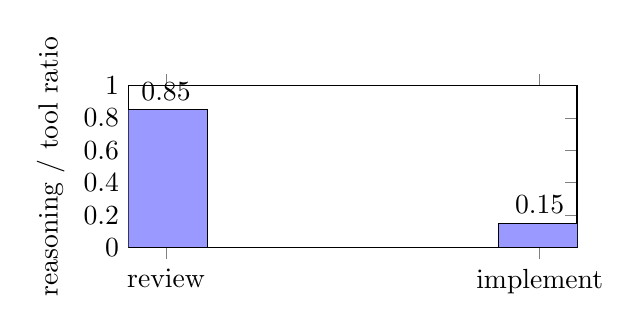
\begin{tikzpicture}
\begin{axis}[
  ybar,
  symbolic x coords={review, implement},
  xtick=data,
  nodes near coords,
  nodes near coords align={vertical},
  ylabel={reasoning / tool ratio},
  ymin=0, ymax=1.0,
  width=0.6\textwidth,
  height=0.3\textwidth,
  bar width=30pt,
]
\addplot[fill=blue!40] coordinates {(review,0.85) (implement,0.15)};
\end{axis}
\end{tikzpicture}
\end{center}

Sessions implementing code show low ratios (0.10--0.20). The high-reasoning sessions are precisely where context rot would manifest: the agent holds massive loaded context that it deliberates over, producing high reasoning per action.

\textbf{Finding 2---Tool Call Size Degradation.} In a single session, tool call sizes degraded from 2,129 bytes (first 50 calls) to 359 bytes (last 50 calls)---an 83\% reduction. This is consistent with either (a) the agent producing more terse tool calls as context degrades, or (b) having less context budget for verbose output. Both indicate context pressure.

\textbf{Finding 3---Cache Hit Ratio.} Across 11 long sessions ($>50$M tokens each), 8 had zero cache hits. The sessions \emph{with} cache hits were those producing patches (file output). Sessions without cache hits were review/approval sessions with high reasoning-per-tool---suggesting the agent loads entirely fresh context on every turn, never reusing cached state.

\textbf{Finding 4---Unfinished Steps.} Across all sessions: 124,744 step-start events vs. 123,328 step-finish events, leaving 1,416 steps that began but never completed. These are direct evidence of interrupted reasoning---context-lost, abandoned mid-cycle, or error-recovery-triggered.

\subsection{Limitations}
The session database stores aggregate token counts, not context snapshots. We cannot directly observe what was in the agent's context at any moment---only the artifacts of what it did with that context. Tool call size is a proxy, not direct evidence. Without intervention studies, correlations do not prove causation.

\section{Why Advisory Enforcement Fails}
\label{sec:why-advisory-fails}

\subsection{The SRD Framework}
Gamage's~\cite{gamage2026} Security-Recall Divergence (SRD) framework provides direct empirical support for our thesis. In a 4,416-trial three-arm causal study across 12 models and 8 providers at 6 conversation depths:

\textbf{Omission (prohibitive) compliance:} 73\% at turn 5 $\to$ 33\% at turn 16. \\
\textbf{Commission (additive) compliance:} 100\% at all turn depths. \\
$p < 10^{-33}$ (Mistral Large 3).

The mechanism is instructive: schema semantic content accounts for 62--100\% of the dilution effect. Re-injecting constraints before the per-model Safe Turn Depth restores compliance---but only if done externally. The model does not self-correct.

\textbf{Implication for the pipe model:} The pipe model's central action---``write artifact to path X before dispatch''---is a commission constraint. Gamage predicts 100\% persistence. The prohibition it replaces---``don't hold intermediate state in context''---is an omission constraint. Gamage predicts decay to 33\% at turn 16. The pipe model converts an omission into a commission.

\subsection{The ``Cost of Compliance''}
Potham~\cite{potham2025} demonstrates that adding a safety principle degrades task success rate even when compliant solutions exist. In his benchmark, TSR dropped from 80\% (no principle) to 14\% (with principle) for a simple detour task. Critically, he also identifies the ``illusion of compliance'': agents appear compliant because they are \emph{incompetent at violating}---not because they choose to follow rules. This confound means that apparent guideline following may mask capability degradation.

\subsection{The Contradiction}
AgentPatterns~\cite{agentpatterns2026instruction} claims positive directives outperform negative ones (``The Pink Elephant Problem''---negatives require the agent to hold the prohibited action in mind while choosing not to act). Zhang et al.~\cite{zhang2026} counters with a large-scale study (679 rule files, 25,532 rules, 5,000+ Claude Code runs) showing that every individually \emph{beneficial} rule is a negative constraint (``do not refactor unrelated code''), while every individually \emph{harmful} rule is a positive directive (``follow code style''). Performance gains are content-independent.

We resolve this contradiction by noting that Zhang studies coding agents with tool access, while Gamage and AgentPatterns study general instruction-following. The pipe model operates at the \emph{orchestration} level---a meta-constraint on the dispatch process itself, not a task-level instruction. This makes it domain-agnostic: routing discipline is separate from task execution. The pipe model is a commission constraint (Gamage predicts persistence) that implements a negative safety constraint (Zhang's PBRS framing---``do not hold temp state in context''). It harmonizes both findings.

\section{Enforcement Strategies: Four Categories}
\label{sec:enforcement}

We classify agent instruction enforcement into four categories, each with distinct failure modes:

\subsection{Model-Level Training (Category 1)}
\textbf{Examples:} OpenAI Instruction Hierarchy~\cite{wallace2024}. Training the model to prioritize instructions by source (system $>$ user $>$ tool output).

\textbf{Failure mode:} Static at deployment. Cannot address runtime context accumulation patterns that emerge only during multi-turn agent operation.

\subsection{Prompt-Level Directives (Category 2)}
\textbf{Examples:} opencode-config guidelines, CLAUDE.md files, system prompt behavioral rules.

\textbf{Failure modes:} Prohibitions decay under context pressure (Gamage: 73\%$\to$33\%). Compliance is often incidental (Potham's ``illusion of compliance''). Gains may be content-independent (Zhang: random rules match curated rules). ``Cost of compliance'' degrades task performance even when compliant solutions exist.

\subsection{Tool-Level Gates (Category 3)}
\textbf{Examples:} MCP tool allowlists, approval gates, policy engines.

\textbf{Failure modes:} Agents respond to tool constraints with value fabrication (inventing plausible-looking values to satisfy parameters), error loops (retrying with slightly different fabricated values until timeout), and bypass seeking (finding alternative pathways that circumvent the gate). No formal academic study of these failure modes exists~\cite{redis2026} documents agents making ``tool calls with hallucinated parameters'' under context pressure, and our session trace reveals 1,416 unfinished steps consistent with error-loop patterns.

\subsection{Architectural Patterns (Category 4)}
\textbf{Examples:} ICM/MWP~\cite{vanclief2026}, Dex Horthy's Research$\to$Plan$\to$Implement workflow~\cite{liu2026}.

\textbf{Failure modes:} Require agent compliance with the architectural pattern. If the agent can skip the discipline step, it reverts to Category 2 (prompt-level directive). The pipe model is a Category 4 strategy that specifically targets context rot from accumulated intermediate state---a gap no existing strategy addresses.

\section{The Filesystem-as-Pipe Model}
\label{sec:model}

\subsection{Core Mechanism}
The pipe model prescribes:

\begin{bluebox}
Before every \texttt{skill()} or \texttt{task()} call:
\begin{enumerate}[nosep]
  \item Write current intermediate state to \texttt{.issues/N/stages/<phase>.md}
  \item Dispatch the call with the artifact path as implicit context
  \item After completion, read only the path to the output artifact from the result contract
  \item The orchestrator NEVER reads artifact content
\end{enumerate}
\end{bluebox}

The orchestrator's context after any dispatch contains exactly:
\begin{enumerate}[nosep]
  \item Path to the previous stage's output artifact
  \item Authorization scope (needed for next routing)
  \item What to call next
\end{enumerate}

The sub-agent reads the artifact from the filesystem independently. The pipe is the routing discipline---not task execution. The agent composes the chain at runtime, adapting to user requests that insert custom steps.

\subsection{Contrast with Current Practice}
Current skill cards contain procedural step-by-step instructions. The agent reads all steps into context (context rot) and then decides which to execute. Under the pipe model, skill cards declare \emph{interfaces}---input schema, output schema, one transformation:

\begin{lstlisting}[style=yaml,caption={Pipe model skill card frontmatter.},label=lst:card]
input_schema:  issues/N/stages/auth-state.yaml
output_schema: issues/N/stages/authorized.yaml
transform: "Verifies authorization scope and labels"
canonical_chain:  # reference pattern, not required execution
  - skill: approval-gate
    output: issues/N/stages/auth-state.yaml
  - task: pre-work
    input: issues/N/stages/auth-state.yaml
    output: issues/N/stages/branch-state.yaml
\end{lstlisting}

The canonical chain is a reference pattern, not a pipeline definition. The agent is free to insert, skip, or reorder steps. The chain emerges from connecting output artifact schemas to input schema requirements.

\subsection{Decomposition to Atomic Steps}
The atomic boundary for a single pipe call is: one input source, one transformation, one output artifact. This mirrors Unix pipe semantics where each command takes one stream and produces one stream---\texttt{grep $\vert$ sort ---} is two calls, two transforms, piped. You do not write \texttt{grep+sort}. You pipe them.

If a stage needs two inputs, it is two calls. If it produces two outputs, it is two calls. The test: ``could this stage be meaningfully executed by a different sub-agent?'' If yes, it is a separate atomic.

\subsection{Composable Agency, Not Static Pipelines}
The pipe model is fundamentally different from graph-based orchestration (LangGraph, CrewAI, DAG frameworks)~\cite{azure2025} where the developer declares the execution graph before runtime. In the pipe model:

\begin{enumerate}[nosep]
  \item No graph is declared. The agent discovers the next stage by matching available artifact schemas against skill card input schemas.
  \item The effective graph emerges from the agent's dispatch decisions---different runs produce different graphs.
  \item State passes through filesystem artifacts at known paths.
  \item The agent composes at runtime---Unix pipeline style, not Makefile style.
\end{enumerate}

This occupies a previously unnamed design space: \textbf{emergent orchestration} (graph discovered at runtime through schema matching) as opposed to \textbf{declarative orchestration} (graph defined at design time). We formalize this distinction as a secondary contribution.

\section{Positioning Within Existing Work}
\label{sec:positioning}

\subsection{Piskala's Framework Extended}
Piskala~\cite{piskala2026} traces the ``everything is a file'' principle from Unix through DevOps to agentic AI, arguing that ``adopting file- and code-centric interaction models may enable agentic systems that are more maintainable, auditable, and operationally robust.'' His framing covers the \emph{agent--world} boundary: agents interact with heterogeneous resources through files.

Our extension covers the \emph{orchestrator--sub-agent} boundary: dispatch stages compose through filesystem artifacts. In Piskala's diagram (Figure~1 in his paper), the evolution goes: Unix $\to$ DevOps $\to$ Agentic AI. Our extension adds: $\to$ Agent Orchestration $\to$ Filesystem-as-Pipe.

\subsection{Comparison with Existing Approaches}
\begin{table}[h]
\centering
\begin{tabular}{lccc}
\toprule
\textbf{Approach} & \textbf{Agent--} & \textbf{Agent--} & \textbf{Dispatch} \\
 & \textbf{World} & \textbf{Memory} & \textbf{Composition} \\
\midrule
Piskala~\cite{piskala2026} & $\checkmark$ & $\checkmark$ & \\
Liu~\cite{liu2026} & $\checkmark$ & $\checkmark$ & \\
Xu/AIGNE~\cite{xu2025} & $\checkmark$ & $\checkmark$ & \\
Turso AgentFS~\cite{turso2025} & & $\checkmark$ & \\
ICM/MWP~\cite{vanclief2026} & & & \\
mcp-dispatch~\cite{sophia2026} & & & $\bigcirc$ \\
\textbf{This paper} & & & $\checkmark$ \\
\bottomrule
\end{tabular}
\caption{Positioning map: the dispatch composition column is empty.}
\label{tab:positioning}
\end{table}

The dispatch composition column is empty in existing work. No prior research theorizes the filesystem as the medium between \texttt{skill()}/\texttt{task()} calls. The closest is Dex Horthy's workflow (cited in Liu~\cite{liu2026}), where a human-designed chain of \texttt{research.md} $\to$ \texttt{plan.md} $\to$ downstream steps creates file boundaries between phases. But Horthy's chain is human-defined and human-triggered. Our model is agent-composed, self-disciplined via mandatory path declaration.

\subsection{Why Ritual Enforcement}
The pipe model is a \textbf{ritual enforcement} mechanism, occupying a middle ground between advisory rules (Category~2, easily ignored) and tool-level gates (Category~3, easily bypassed or broken). Ritual enforcement is:

\begin{enumerate}[nosep]
  \item Not a tool constraint---no fabrication triggers, no error loops.
  \item Not a prohibition---positive action, step-wise check-listable.
  \item Creates an artifact trail---violations leave evidence (missing artifacts).
  \item Self-reinforcing---each stage's artifact is required by the next stage's input.
\end{enumerate}

It is an architectural (Category~4) strategy that requires no agent runtime modifications. The discipline lives entirely in skill card design and guideline patterns.

\subsection{Pipeline Model}

\begin{center}
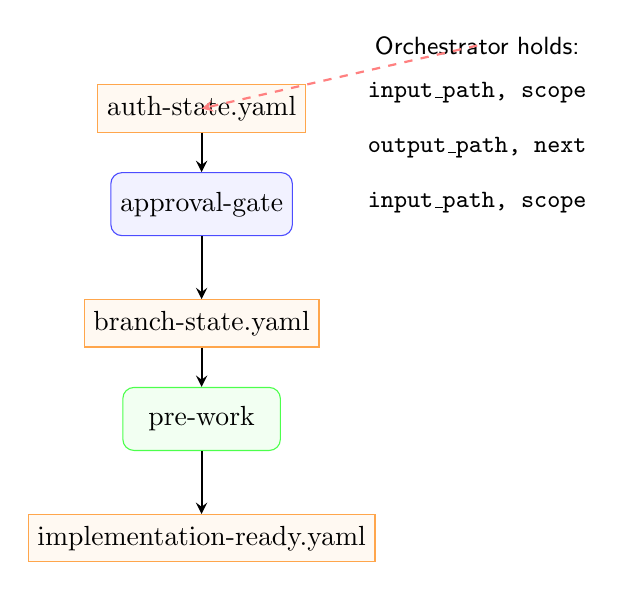
\begin{tikzpicture}[
  node distance=0.5cm and 1cm,
  skill/.style={rectangle, draw=blue!70, fill=blue!5, rounded corners, minimum width=2cm, minimum height=0.8cm},
  task/.style={rectangle, draw=green!70, fill=green!5, rounded corners, minimum width=2cm, minimum height=0.8cm},
  artifact/.style={rectangle, draw=orange!70, fill=orange!5, minimum width=2.5cm, minimum height=0.6cm},
  pipe/.style={draw, ->, >=stealth, thick},
  context/.style={draw, dashed, ->, >=stealth, thick, color=red!50},
]
\node[artifact] (a1) at (0,0) {auth-state.yaml};
\node[skill] (s1) [below=of a1] {approval-gate};
\node[artifact] (a2) [below=of s1, yshift=-0.3cm] {branch-state.yaml};
\node[task] (t1) [below=of a2] {pre-work};
\node[artifact] (a3) [below=of t1, yshift=-0.3cm] {implementation-ready.yaml};

\draw[pipe] (a1) -- (s1);
\draw[pipe] (s1) -- (a2);
\draw[pipe] (a2) -- (t1);
\draw[pipe] (t1) -- (a3);

% annotate
\node[align=center, font=\small\sffamily] at (3.5, 0.8) {Orchestrator holds:};
\node[align=left, font=\small\ttfamily] at (3.5, 0.2) {input\_path, scope};
\node[align=left, font=\small\ttfamily] at (3.5, -0.5) {output\_path, next};
\node[align=left, font=\small\ttfamily] at (3.5, -1.2) {input\_path, scope};

\draw[context] (3.5, 0.8) -- (0, 0);
\end{tikzpicture}
\end{center}

\section{Limitations and Future Work}
\label{sec:limitations}

\subsection{Known Failure Modes}
The pipe model has known failure modes the paper must acknowledge:

\begin{enumerate}[nosep]
  \item \textbf{Corrupt artifacts:} Sub-agent writes malformed data to artifact path. Next stage reads garbage. No schema validation exists at the tool level---the pipe model has no type checking.
  \item \textbf{Path collisions:} Two concurrent sessions write to the same path. Mitigation: include issue number and timestamp in path.
  \item \textbf{Artifact path fabrication:} Agent invents a path that does not exist. This is the same as the general ``agent fabricates values'' problem---not specific to the pipe model.
  \item \textbf{Ritual discipline failure:} Under high cognitive load (error recovery, complex user request), the agent skips the artifact write. However, if the artifact is missing, the next stage fails fast---the discipline is self-enforcing through stage dependency.
  \item \textbf{Stage boundary mismatch:} Agent decomposes a task differently than the skill card's canonical chain. Schema mismatch detection is the mitigation.
\end{enumerate}

\subsection{Threats to Validity}
Our empirical evidence is from session traces of a single agent system (opencode). While the database contains 6,764 sessions across diverse tasks, generalizing to other agent frameworks requires caution. The tool call size degradation finding (2,129$\to$359 bytes) is from a single session and may not generalize.

The ``ritual enforcement'' claim lacks intervention studies. We have shown that prohibitions decay (Gamage's SRD) and that positive actions persist (same study). We have not measured whether the pipe model's specific positive action---``write artifact to path before dispatch''---persists at the same rate as Gamage's commission constraints. This requires a controlled experiment.

\subsection{Future Work}
\label{sec:future}
\begin{enumerate}[nosep]
  \item \textbf{Intervention study:} Implement pipe guidelines in a skill deck, run behavioral test suite comparing current (advisory) vs. pipe (ritual) context discipline.
  \item \textbf{Empirical validation of context rot metrics:} Reasoning-per-tool ratio, tool call size degradation rate, cache hit ratio, and unfinished step count as measurable indicators.
  \item \textbf{Schema-based artifact validation:} Define minimum viable artifact schema---what guarantees that stage N's output is consumable by stage N+1.
  \item \textbf{Generalization to other agent frameworks:} Test the pipe model in LangGraph, CrewAI, and other orchestration frameworks.
  \item \textbf{Cache hit prediction:} If the pipe model creates stable artifact paths across dispatches, cache hit ratios should increase. This is a testable prediction from our Finding~3.
\end{enumerate}

\section{Conclusion}
\label{sec:conclusion}

AI agents accumulate context rot---intermediate state from prior dispatch stages that persists past its useful lifetime, degrading compliance and decision quality. Advisory guidelines prohibiting this fail: omission constraints decay from 73\% to 33\% over 16 turns, while commission constraints persist at 100\%. The filesystem-as-pipe model converts an omission into a commission---``write artifact to path X before each dispatch''---a ritual discipline enforced by the agent's own positive action, not by tool-level gates or code changes to the agent runtime.

This extends Piskala's ``files-are-all-you-need'' framework from the agent--world interface (files as the medium of interaction) to the orchestration layer (files as the medium of composition between dispatch stages). The dispatch composition column is empty in the literature. The pipe model fills it.

We have presented empirical evidence from a 4.1~GB session trace of 6,764 real agent sessions---revealing patterns consistent with context rot: 83\% tool call size degradation, 1,416 unfinished reasoning steps, near-zero cache hit ratios in long sessions. We have classified four enforcement strategy categories and shown the gap the pipe model fills. We have named a previously untheorized design space---declarative vs.\ emergent orchestration.

The pipe model requires no agent runtime modifications. It lives entirely in skill card design and guideline patterns. It is deployable today.

\begin{thebibliography}{99}

\bibitem{gamage2026}
Y.\ Gamage.
``Omission Constraints Decay While Commission Constraints Persist in Long-Context LLM Agents.''
arXiv:2604.20911, Apr.\ 2026.

\bibitem{potham2025}
R.\ Potham.
``Evaluating LLM Agent Adherence to Hierarchical Safety Principles.''
ICML 2025 Technical AI Governance Workshop, arXiv:2506.02357.

\bibitem{piskala2026}
D.\ B.\ Piskala.
``From Everything-is-a-File to Files-Are-All-You-Need: How Unix Philosophy Informs the Design of Agentic AI Systems.''
arXiv:2601.11672, Jan.\ 2026.

\bibitem{tianpan2026}
T.\ Pan.
``Context Poisoning in Long-Running AI Agents.''
tianpan.co, Apr.\ 2026.

\bibitem{redis2026}
J.\ A.\ Wallace.
``Context Poisoning: How Bad Information Breaks Agent Reasoning.''
Redis Blog, May 2026.

\bibitem{agentpatterns2026}
AgentPatterns.tech.
``Context Poisoning: When Agent Context Becomes Unreliable.''
2026.

\bibitem{agentpatterns2026instruction}
AgentPatterns.tech.
``Instruction Polarity: Positive vs.\ Negative Directives.''
2026.

\bibitem{zhang2026}
X.\ Zhang, G.\ Wang, Y.\ Cui, W.\ Qiu, Z.\ Li, B.\ Zhu, P.\ He.
``Guardrails Beat Guidance: A Large-Scale Study of Rules, Skills, and Persistent Configuration for Coding Agents.''
arXiv:2604.11088, Apr.\ 2026.

\bibitem{wallace2024}
E.\ Wallace, K.\ Xiao, R.\ Leike, L.\ Weng, J.\ Heidecke, A.\ Beutel.
``The Instruction Hierarchy: Training LLMs to Prioritize Privileged Instructions.''
arXiv:2404.13208, Apr.\ 2024.

\bibitem{liu2026}
J.\ Liu.
``Files Are All You Need.''
LlamaIndex Blog, Jan.\ 2026.

\bibitem{xu2025}
X.\ Xu, R.\ Mao, Q.\ Bai, X.\ Gu, Y.\ Li, L.\ Zhu.
``Everything is Context: Agentic File System Abstraction for Context Engineering.''
AIGNE Framework, arXiv:2512.05470, Dec.\ 2025.

\bibitem{vanclief2026}
J.\ Van Clief, D.\ McDermott.
``Interpretable Context Methodology: Folder Structure as Agentic Architecture.''
arXiv:2603.16021, Mar.\ 2026.

\bibitem{opencode2026}
anomalyco/opencode.
``Session SQL Schema.''
GitHub, packages/opencode/src/session/session.sql.ts, 2026.

\bibitem{turso2025}
P.\ Enberg, G.\ Costa.
``The Missing Abstraction for AI Agents: The Agent Filesystem.''
Turso Blog, Nov.\ 2025.

\bibitem{sophia2026}
sophia-labs/mcp-dispatch.
``Local Inter-Agent Messaging for AI Coding Agents via MCP.''
GitHub, 2026.

\bibitem{azure2025}
Microsoft Azure Architecture Center.
``AI Agent Orchestration Patterns.''
2025.

\end{thebibliography}

\vspace{0.5cm}
\noindent\textit{Co-authored with AI: OpenCode (deepseek-v4-flash)}

\end{document}
